\documentclass{math_hw}
\usepackage{cleveref}
\usepackage{amsthm}
\usepackage{bm}
%\usepackage{subfigure}
\usepackage{subcaption}
\renewcommand\qedsymbol{\blacksquare}


\onehalfspacing
\theoremstyle{definition}
\newtheorem{definition}{Definition}[section]

\title{\textbf{Homework 1}\\ \vspace{1em}
MATH 578: Intro to Numerical PDEs}
\author[1]{Liam Pohlmann}
%\author[2]{Someone else\ldots}
\affil[1]{University of New Mexico, Department of Nuclear Engineering}
%\affil[2]{University of New Mexico, Department of \ldots}

\date{\textbf{Due: 11 February 2024}}

\begin{document}
    \maketitle
    \tableofcontents
    \clearpage


    \section*{Premise}
    In this assignment, we look to analyze the consistency and stability of three finite difference schemes, which are:
    \begin{enumerate}
        \item Forward Time Backward Space: \begin{equation}
                                               \tag{A} \label{scheme A}
                                               v^{n+1}_i = (1-\lambda)v_i^n+\lambda v_{i-1}^n
        \end{equation}
        \item Lax-Friedrichs: \begin{equation}
                                  \tag{B} \label{scheme B}
                                  v_i^{n+1} = \frac{1}{2}(1-\lambda)v_{i+1}^n + \frac{1}{2}(1+\lambda)v_{i-1}^n
        \end{equation}
        \item Leap-Frog: \begin{equation}
                             \tag{C} \label{scheme C}
                             v_1^{n+1} = v_i^{n-1}-\lambda v_{i+1}^n +\lambda v_{i-1}^n
        \end{equation}
    \end{enumerate}
    These schemes are implemented as solutions to the diffusion equation:
    \begin{equation}
        u_t +u_x = 0 \quad t\geq 0, \quad x\in [-1,1]
    \end{equation}
    with the initial condition:
    \begin{equation*}
        u(0,x) = f(x) = \begin{cases}
                            f_1(x) = \begin{cases}
                                         1& -0.5\leq x \leq 0.5 \\
                                         0 & \text{elsewhere}
                            \end{cases} \\
                            f_2(x) = \sin(2\pi x)
        \end{cases}
        \quad t=0,\quad x\in [-1,1]
    \end{equation*}
    and \textit{periodic} boundary conditions:
    \begin{equation*}
        u(t,-1)=u(t,1),\quad t>0
    \end{equation*}
    The solutions to this equation are simply:
    \begin{equation} \label{u_exact}
        u(t,x) = f(x-t)
    \end{equation}
    where $f$ is the initial condition as stated above.

    Additionally, we specify \textit{uniform} spacing in both $x$ and $t$ such that $h=\Delta x$, $k=\Delta t$ and $\lambda = \nicefrac{k}{h}$.
    Lastly, we note that $v_i^n\approx u(ih,nk)$ for $i=-M,-M+1,\ldots,M-1,M$ and $n=0,1,\ldots,N$.

    For convenience, we rewrite \cref{scheme A,scheme B,scheme C} as:
    \begin{equation}
        \label{scheme A'}
        \tag{A'}
        0=(1-\lambda)v_i^n+\lambda v_{i-1}^n-v^{n+1}_i
    \end{equation}
    \begin{equation}
        \label{scheme B'}
        \tag{B'}
        0=\frac{1}{2}(1-\lambda)v_{i+1}^n + \frac{1}{2}(1+\lambda)v_{i-1}^n-v^{n+1}_i
    \end{equation}
    \begin{equation}
        \label{scheme C'}
        \tag{C'}
        0=v_i^{n-1}-\lambda v_{i+1}^n +\lambda v_{i-1}^n-v^{n+1}_i
    \end{equation}


    \section{Show that all three schemes are consistent with the advection equation.}
    \begin{definition}[Consistency]\label{eq:consistency}
        A finite difference scheme is \textit{consistent} if
        \begin{equation}
            P\phi -P_{k,i}\phi \xrightarrow{h,k\to 0} 0.
        \end{equation}
    \end{definition}

    Using Taylor's expansion, the following are derived:
    \begin{equation}
        \phi_i^{n+1} = \phi_i^n +k\phi_t + \mathcal{O}(k^2)
    \end{equation}
    \begin{equation}
        \phi_i^{n+1} = \phi_i^n -h\phi_x + \mathcal{O}(h^2)
    \end{equation}
    and
    \begin{equation}
        \phi_i^{n+1} = \phi_i^n+h\phi_x+\mathcal{O}(h^2)
    \end{equation}

    \subsection*{Scheme~\ref{scheme A}:}
    \begin{equation}
        \label{eq:scheme-a-discrete-consistency}
        \begin{split}
            P_{k,i}\phi &=(1-\lambda) \phi_i^n +\lambda \phi_{i-1}^n-\phi_i^{n+1} \\
            &= (1-\lambda)\phi_i^n+\lambda \left( \phi_i^n-h\phi_x+\mathcal{O}(h^2) \right) - \left( \phi_i^n+k\phi_t+\mathcal{O}(k^2) \right)\\
            &=-h\lambda \phi_x + \lambda\mathcal{O}(h^2) -k\phi_t+\mathcal{O}(k^2)\\
            &= -k\phi_x+k\mathcal{O}(h)-k\phi_t+\mathcal{O}(k^2) = 0
        \end{split}
    \end{equation}
    By dividing \cref{eq:scheme-a-discrete-consistency} by $k$ and substituting into \cref{eq:consistency}, we find:
    \begin{equation*}
    (\phi_t+\phi_x)
        - \left( \phi_t+\phi_x+\mathcal{O}(h) + \mathcal{O}(k) \right) =\mathcal{O}(h) + \mathcal{O}(k)\xrightarrow{h,k\to 0} 0 \quad \qedsymbol
    \end{equation*}

    \subsection*{Scheme~\ref{scheme B}:}
    \begin{equation}
        \label{eq:scheme-b-discrete-consistency}
        \begin{split}
            P_{k,i}\phi &= \frac{1}{2}\left( 1-\lambda \right)\phi_{i+1}^n+\frac{1}{2}\left( 1+\lambda \right)\phi_{i-1}^n-\phi_i^{n+1} \\
            &= \frac{1}{2}(1-\lambda)\left( \phi_i^n+h\phi_x+\mathcal{O}(h^2) \right)+\frac{1}{2}(1+\lambda)\left( \phi_i^n-h\phi_x+\mathcal(O)(h^2) \right) +\\ &\quad - \left( \phi_i^n+k\phi_t+\mathcal(O)(k^2) \right) \\
            &=\phi_i^n-\lambda h\phi_x+\mathcal{O}(h^2)-\phi_i^n-k\phi_t+\mathcal{O}(k^2)\\
            &= -k\phi_x-k\phi_t+\mathcal{O}(h^2)+\mathcal{O}(k^2) = 0
        \end{split}
    \end{equation}
    Dividing \cref{eq:scheme-b-discrete-consistency} by $k$, then applying \cref{eq:consistency}, we find:
    \begin{equation*}
        \phi_x+\phi_t-\left( \phi_x+\phi_t + \mathcal{O}\left(\frac{h^2}{k}\right) + \mathcal{O}(k)\right) = \mathcal{O}\left(\frac{h^2}{k}\right) + \mathcal{O}(k)\xrightarrow{h,k\to 0} 0 \quad \qedsymbol
    \end{equation*}
    Although $k$ remains in the denominator, we argue that as both $h$ and $k$ approach 0, the numerator decreases more rapidly due to its quadratic nature.
    Thus, all error terms will go to 0, showing that the scheme is consistent by \cref{eq:consistency}.

    \subsection*{Scheme~\ref{scheme C}}
    \textit{Note: The Taylor expansions about $\phi_i^{n\pm 1}$ have been expanded further to include the quadratic. This adds $\frac{k^2}{2}\phi_{tt}$ to each, changing the final term to $\mathcal{O}(k^3)$.}
    \begin{equation}
        \label{eq:scheme-c-consistency}
        \begin{split}
            P_{k,i}\phi &= \phi_i^{n-1}-\lambda\phi_{i+1}^n+\lambda\phi_{i-1}-\phi_i^{n+1}\\
            &=\phi_i^n-k\phi_t+\frac{k^2}{2}\phi_{tt}+\mathcal{O}(k^3)-\lambda\left( \phi_i^n+h\phi_x+\mathcal{O}(h^2) \right) +\\ &\quad + \lambda\left( \phi_i^n-h\phi_x+\mathcal{O}(h^2) \right) - \left( \phi_i^n+k\phi_t+\frac{k^2}{2}\phi_{tt}+\mathcal{O}(k^3) \right) \\
            &=-2k\phi_t-2\lambda h\phi_x+\mathcal{O}(k^3)+k\mathcal{O}(h)+\mathcal{O}(h^2)=0
        \end{split}
    \end{equation}
    By dividing \cref{eq:scheme-c-consistency} by $-2k$ and substituting into \cref{eq:consistency}, we find:
    \begin{equation*}
        \phi_t+\phi_x-\left( \phi_t+\phi_x+\mathcal{O}(k^2)+\mathcal{O}(h) +\mathcal{O}\left(\frac{h^2}{k}\right) \right) = \mathcal{O}(k^2)+\mathcal{O}(h)+\mathcal{O}\left(\frac{h^2}{k}\right)\xrightarrow{h,k\to 0} 0 \quad \qedsymbol
    \end{equation*}


    \section{{State the CFL condition, and show that \textbf{A} and \textbf{B} are stable if the CFL condition is satisfied.}} \label{sec:q2}
    In analyzing the stability of a finite-difference scheme, the Fourier Transform lends itself as a valuable tool.
    Circumventing lengthy derivation, we will simply replace the approximated solution, $v_j^n$ with $g^n \cdot e^{ij\theta}$, where $g$ is the growth factor and $i=\sqrt {-1}$. $j$ is the index in space.
    The CFL condition is then greatly simplified to:
    \begin{equation}
        \label{eq:cfl-condition}
        \left\| g(\theta,h,k) \right\|^2 \leq \left( 1+Ck \right)^2
    \end{equation}
    where $C$ is a constant.

    \subsection*{Scheme~\ref{scheme A}:}
    Beginning with \cref{scheme A'}, we replace $v_j^n$ with $g^n \cdot e^{ij\theta}$, then simplify to find:
    \begin{equation*}
        \label{2A'}
        \begin{split}
            0&= (1-\lambda)g^n e^{ij\theta} +\lambda g^n e^{i(j-1)\theta} -\underbrace{g^{n+1}}_{=g^n\cdot g} e^{ij\theta} \\
            &=g^n e^{ij\theta} \underbrace{\left(1-\lambda +\lambda e^{-i\theta}-g\right)}_{\text{This must equal 0}}
        \end{split}
    \end{equation*}
    Solving for $g$ in the braced expression gives:
    \begin{equation*}
        \label{2A g}
        \begin{split}
            g &= 1-\lambda +\lambda e^{-i\theta}\\
            &= 1-\lambda+\lambda(\cos\theta -i\sin\theta)\\
            &=1-\lambda +\lambda\cos \theta -\lambda i\sin \theta
        \end{split}
    \end{equation*}
    Applying \cref{eq:cfl-condition}:
    \begin{equation*}
        \begin{split}
            \left\| g \right\|^2 &= \left( 1-\lambda +\lambda\cos \theta \right)^2 + \left( \lambda i\sin \theta \right)^2\\
            &= 1-2\lambda +2\lambda \cos \theta +\lambda^2 -2\lambda ^2 \cos \theta +\lambda ^2 \underbrace{\left( \cos^2 \theta +\sin^2\theta \right)}_{=1}
        \end{split}
    \end{equation*}
    Using the fact that $\cos \theta \leq 1$, all terms above cancel, leaving:
    \begin{equation*}
        \left\| g \right\|^2 =1 \leq 1 \quad \qedsymbol
    \end{equation*}

    \subsection*{Scheme~\ref{scheme B}:}
    Following a similar procedure to Scheme~\ref{scheme B}, we find:
    \begin{equation*}
        \begin{split}
            0 &= \frac{1}{2}(1-\lambda)g^{n}e^{i(j+1)\theta}+\frac{1}{2} (1+\lambda)g^{n}e^{i(j-1)\theta}-g^n\cdot g e^{ij\theta} \\
            &=g^n e^{ij\theta}\underbrace{\left[ \frac{1}{2}(1-\lambda)e^{i\theta}+\frac{1}{2}(1+\lambda)e^{-i\theta} -g \right]}_{\text{must equal 0}}
        \end{split}
    \end{equation*}
    Solving for $g$ yields:
    \begin{equation*}
        \begin{split}
            g&=\frac{1}{2}\left( e^{i\theta}+e^{-i\theta} \right)-\frac{1}{2}\lambda\left( e^{i\theta}-e^{-i\theta} \right)\\
            &=\cos \theta -\lambda i\sin \theta
        \end{split}
    \end{equation*}
    Applying \cref{eq:cfl-condition} gives:
    \begin{equation*}
        \begin{split}
            \left\| g \right\|^2 &= \cos^2\theta +\lambda ^2\sin ^2 \theta \\
            &=1-\sin ^2 \theta \left( 1-\lambda ^2 \right),\quad \sin^2 \theta \leq 1 \\ \\
            \text{so:}\quad \left\| g \right\|^2 &\leq \lambda^2 \leq \left( 1+Ck \right)^2 \quad \qedsymbol
        \end{split}
    \end{equation*}


    \section{{State a necessary condition for \textbf{C} to be stable.}} \label{sec:q3}
    To determine the stability of \cref{scheme C}, we will follow the same procedure as seen in \cref{sec:q2}.
    Replacing $v_i^n$ with $g^n e^{ij\theta}$ for \cref{scheme C'}, we find:
    \begin{equation*}
        \begin{split}
            0&= g^{n-1}e^{ij\theta} -\lambda g^n e^{i(j+1)\theta}+\lambda g^{ne^{i(j-1)\theta}}-g\cdot g^n e^{ij\theta} \\
            \text{Write in terms of $g^{n-1}$:} \quad &=g^{n-1}e^{ij\theta} -\lambda g\cdot g^{n-1} e^{i(j+1)\theta}+\lambda g\cdot g^{n-1}e^{i(j-1)\theta}-g\cdot g^2 \cdot g^{n-1} e^{ij\theta}\\
            &= g^{n-1}e^{ij\theta}\underbrace{\left( 1-\lambda ge^{i\theta}+\lambda g^{-i\theta}-g^2 \right)}_{\text{must equal 0}}
        \end{split}
    \end{equation*}
    Solving for $g$ gives:
    \begin{equation*}
        \begin{split}
            0 &=1-g^2-\lambda g\left( e^{i\theta}-e^{-i\theta} \right) \\
            &=g^2 + 2\lambda ig\sin \theta -1
        \end{split}
    \end{equation*}
    To solve, we complete the square and simplify.
    \begin{equation*}
        \begin{split}
            \quad g^2 + 2\lambda ig\sin \theta +\left( \lambda i\sin \theta \right)^2 &= 1+ \left( \lambda i\sin \theta \right)^2 \\
            \left( g+\lambda i\sin \theta \right)^2 &= 1-\lambda^2\sin ^2 \theta \\
            g &= -\lambda i\sin \theta \pm \sqrt {1-\lambda^2 \sin^2 \theta }
        \end{split}
    \end{equation*}
    The sign of the discriminant is quite important to the analysis, as it determines how much we can say regarding the stability.
    If it is negative, we observe:
    \begin{equation*}
        \begin{split}
            \left\| g \right\|^2 &= \left( -\lambda\sin \theta \pm \sqrt {\lambda^2\sin ^2 \theta -1} \right)^2 \\
            &= 2\lambda^2 \sin ^2\theta \mp 2\sqrt {\lambda^2 \sin^2 \theta -1} -1
        \end{split}
    \end{equation*}
    which bounds both $\theta$ and $\lambda$.
    However, if we demand the discriminant to be strictly positive, then we find:
    \begin{equation*}
        \begin{split}
            \left\| g \right\|^2 &= 1 - \lambda^2 \sin^2 \theta +\lambda^2 \sin^2 \theta\\
            &= 1 \leq \left( 1+Ck \right)^2
        \end{split}
    \end{equation*}
    showing that we are \textit{unconditionally} stable.
    This condition can be simplified by realizing $\sin^2\theta \leq 1$, giving:
    \begin{equation*}
        \begin{split}
            1-\lambda^2\sin^2 \theta &>0\\
            \Rightarrow \quad  1&>\lambda^2 \sin^2 \theta \\
            &> \lambda ^2
        \end{split}
    \end{equation*}
    \textbf{Therefore, for Scheme C to be guaranteed stable, we demand that $\boldsymbol{{\lambda}^2<1}$.}
    Because $\lambda > 0$, it is synonymous to demand $\lambda <1$.


    \section{Implementation}
    All three schemes (\cref{scheme A,scheme B,scheme C}) were implemented with $\lambda = [0.5,0.8,1,2]$, and the solutions at $t=2$ are reported for $f_1$ in \cref{f1 figures} and $f_2$ in \cref{f2 figures}.

For all cases, the solutions matched well with the theory derived above. 
That is, all schemes were proven to be stable.
Although the error\footnote{The discrete L2 norm was reported on each subfigure for reference, calculated using the Trapezoid Rule.} grew quite large for $\lambda =2$ in \textit{all} cases, the solutions did \textit{not} go to $\pm \infty$ in finite time.
In this case, we deduce that not all $\lambda$ values are applicable to solving a PDE.

Generally, the error reduced for each scheme as $\lambda \rightarrow 1$, aside from \cref{weird leap frog}, indicating a convergence of error as $k\rightarrow h$.
However, the error grows rapidly once $k>h$.
\Cref{weird leap frog} can be explained by the results in~\cref{sec:q3}, where the scheme may become unstable when $\lambda \geq 1$ (this point can be thought of as a bifurcation in stability analysis), which is supported by the many orders of magnitude difference between Scheme \textbf{C} and Schemes \textbf{A} and \textbf{B} once $\lambda =2$.
Overall, it appears clear that Forward-Time-Backward-Space (FTBS) and Leap-Frog were the best methods in terms of accuracy and convergence to their respective best numerical answer.
However, it appears that FTBS performed better overall, as it avoided much of the ``wobbling'' observed by the Leap-Frog scheme.
That said, Leap-Frog appears much better suited for solving continuous, smooth schemes, even at lower $\lambda$ values, implying that a less-fine spatial discretization could be used, which would speed up the computation.
\\ \\
\noindent \textit{Note:} Because Scheme \textbf{C} depends on the previous \textit{two} time steps, the first time step taken after the initial conditions is found using Scheme \textbf{A}.
Additionally, the code was created such that the periodic boundary condition was satisfied for $f_1$ by demanding $x-t\in [-1,1]$.
This was achieved by creating a \texttt{while} loop which shifts the input by the length of the interval (in this case, by adding 2).
Python code is available upon request by contacting \url{lipohlmann@unm.edu}.

\begin{figure}
    \centering
    \begin{subfigure}{0.3\linewidth}
        \centering
        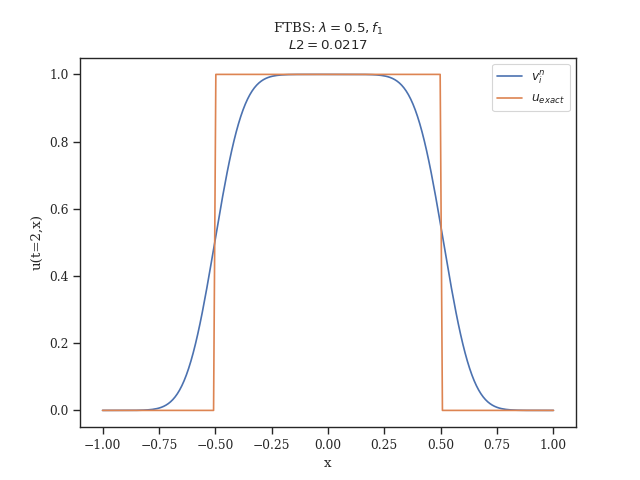
\includegraphics[width=\linewidth]{figures/FTBS/FTBS_lambda=0.5,f1}
        \caption{FTBS, $\lambda = 0.5$}
    \end{subfigure}
    \hfill
    \begin{subfigure}{0.3\linewidth}
        \centering
        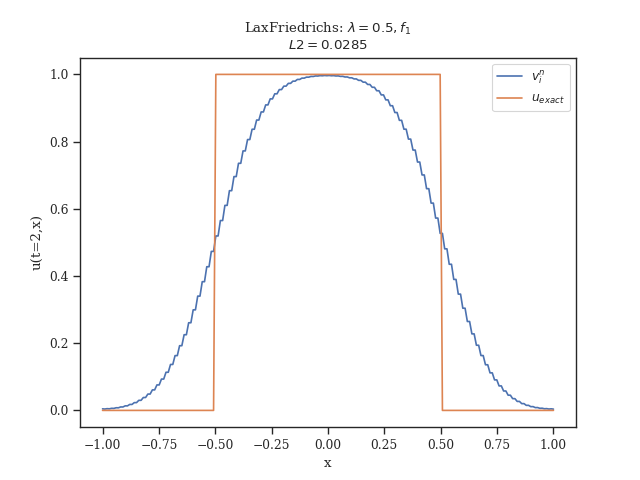
\includegraphics[width=\linewidth]{figures/LaxFriedrichs/LaxFriedrichs_lambda=0.5,f1}
        \caption{Lax-Friedrichs, $\lambda =0.5$}
    \end{subfigure}
    \hfill
    \begin{subfigure}{0.3\linewidth}
        \centering
        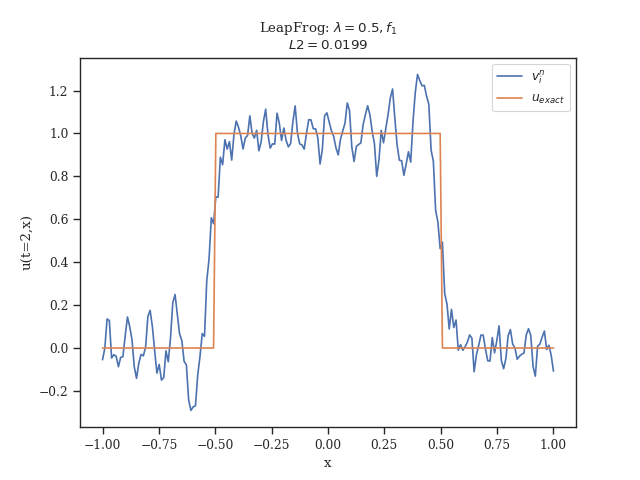
\includegraphics[width=\linewidth]{figures/LeapFrog/LeapFrog_lambda=0.5,f1}
        \caption{Leap-Frog, $\lambda =0.5$}
    \end{subfigure}
    \hfill
    \vspace{1cm}
    \begin{subfigure}{0.3\linewidth}
        \centering
        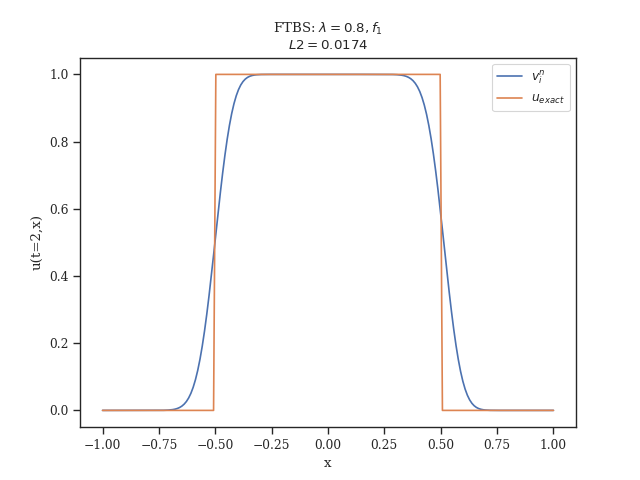
\includegraphics[width=\linewidth]{figures/FTBS/FTBS_lambda=0.8,f1}
        \caption{FTBS, $\lambda = 0.8$}
    \end{subfigure}
    \hfill
    \begin{subfigure}{0.3\linewidth}
        \centering
        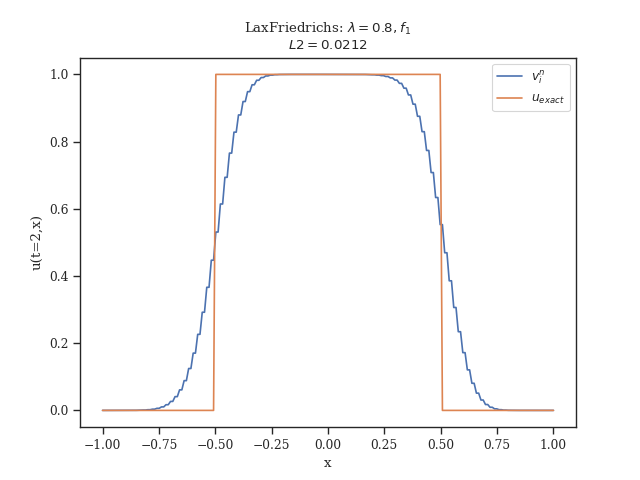
\includegraphics[width=\linewidth]{figures/LaxFriedrichs/LaxFriedrichs_lambda=0.8,f1}
        \caption{Lax-Friedrichs, $\lambda =0.8$}
    \end{subfigure}
    \hfill
    \begin{subfigure}{0.3\linewidth}
        \centering
        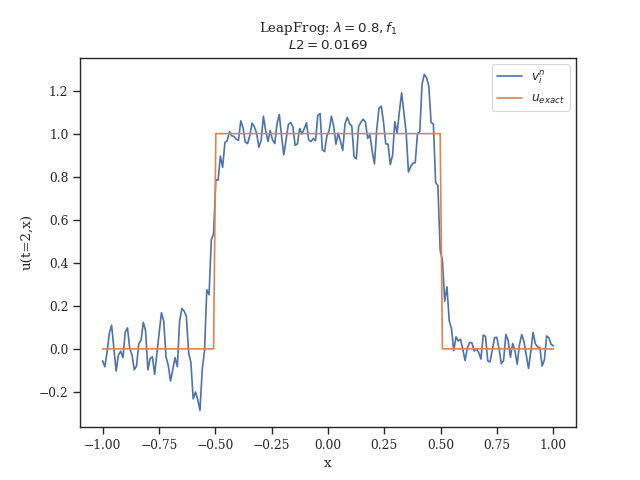
\includegraphics[width=\linewidth]{figures/LeapFrog/LeapFrog_lambda=0.8,f1}
        \caption{Leap-Frog, $\lambda =0.8$}
    \end{subfigure}
    \hfill
    \vspace{1cm}
    \begin{subfigure}{0.3\linewidth}
        \centering
        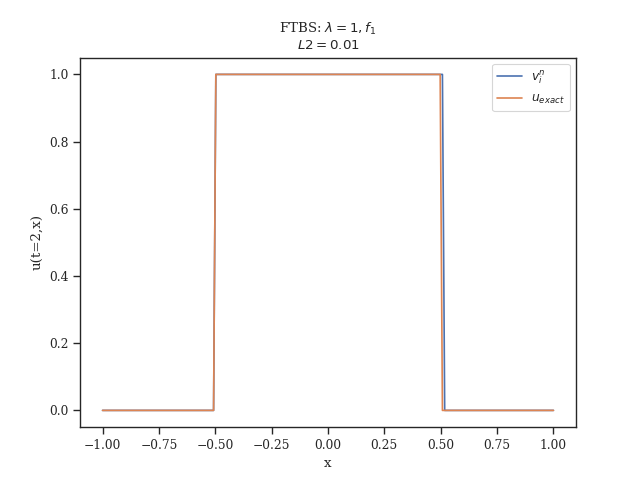
\includegraphics[width=\linewidth]{figures/FTBS/FTBS_lambda=1,f1}
        \caption{FTBS, $\lambda = 1$}
    \end{subfigure}
    \hfill
    \begin{subfigure}{0.3\linewidth}
        \centering
        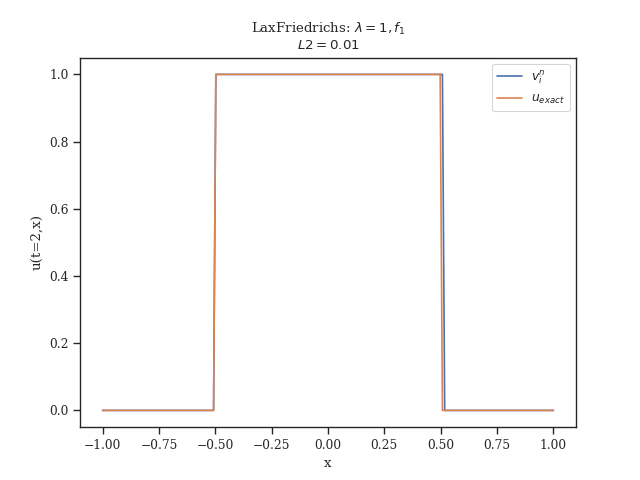
\includegraphics[width=\linewidth]{figures/LaxFriedrichs/LaxFriedrichs_lambda=1,f1}
        \caption{Lax-Friedrichs, $\lambda =1$}
    \end{subfigure}
    \hfill
    \begin{subfigure}{0.3\linewidth}
        \centering
        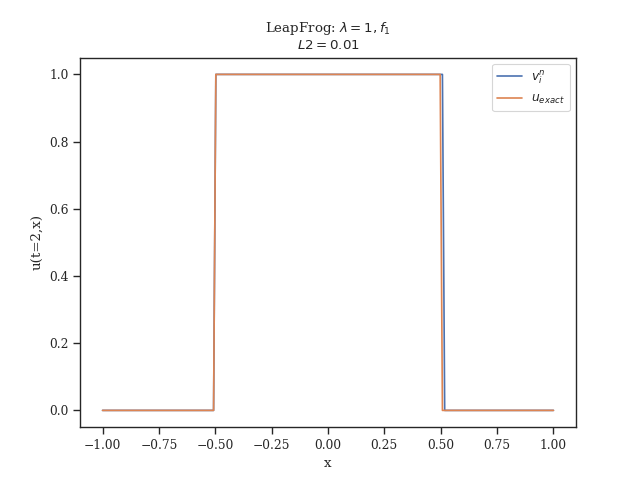
\includegraphics[width=\linewidth]{figures/LeapFrog/LeapFrog_lambda=1,f1}
        \caption{Leap-Frog, $\lambda =1$}
    \end{subfigure}
    \hfill
    \vspace{1cm}
    \begin{subfigure}{0.3\linewidth}
        \centering
        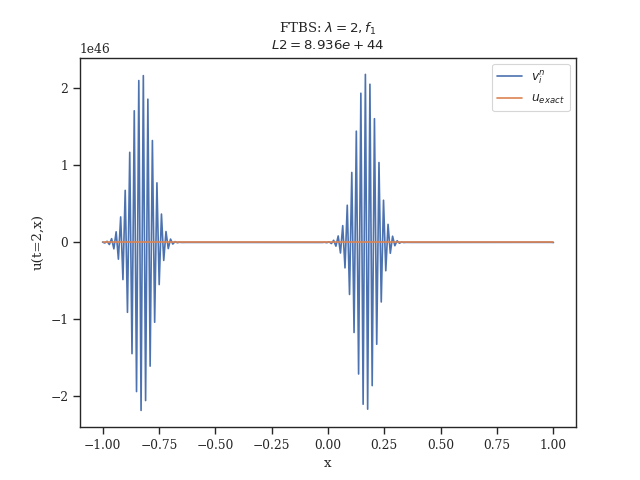
\includegraphics[width=\linewidth]{figures/FTBS/FTBS_lambda=2,f1}
        \caption{FTBS, $\lambda = 2$}
    \end{subfigure}
    \hfill
    \begin{subfigure}{0.3\linewidth}
        \centering
        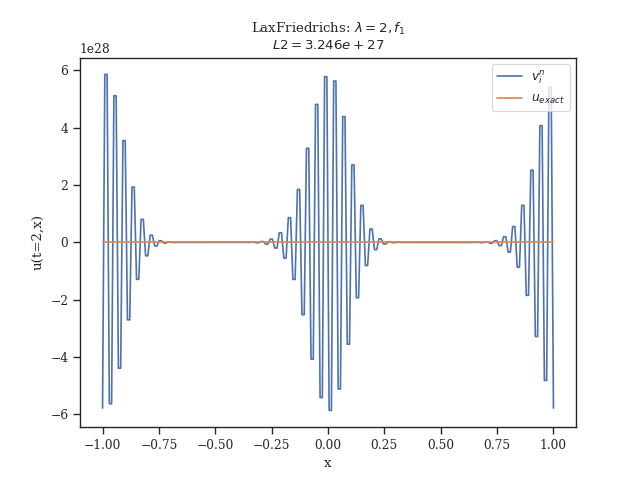
\includegraphics[width=\linewidth]{figures/LaxFriedrichs/LaxFriedrichs_lambda=2,f1}
        \caption{Lax-Friedrichs, $\lambda =2$}
    \end{subfigure}
    \hfill
    \begin{subfigure}{0.3\linewidth}
        \centering
        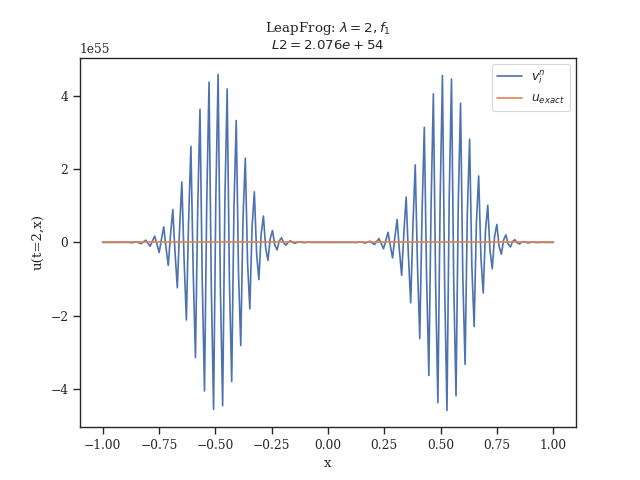
\includegraphics[width=\linewidth]{figures/LeapFrog/LeapFrog_lambda=2,f1}
        \caption{Leap-Frog, $\lambda =2$}
    \end{subfigure}
    \hfill

    \caption{Solutions of Varying $\lambda$ for $f_1$}
    \label{f1 figures}

\end{figure}

\begin{figure}
    \centering
    \begin{subfigure}{0.3\linewidth}
        \centering
        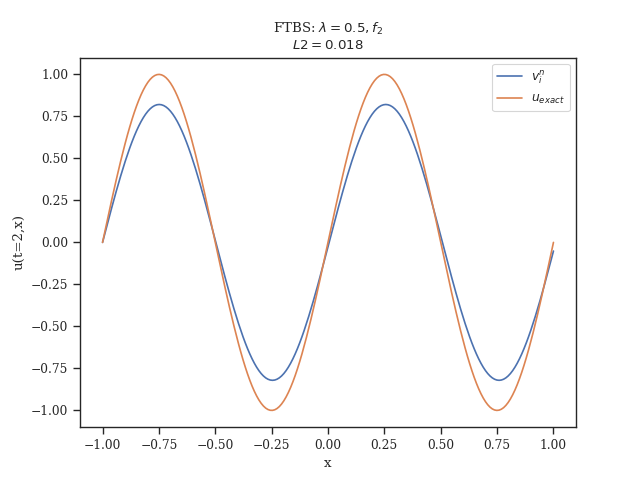
\includegraphics[width=\linewidth]{figures/FTBS/FTBS_lambda=0.5,f2}
        \caption{FTBS, $\lambda = 0.5$}
    \end{subfigure}
    \hfill
    \begin{subfigure}{0.3\linewidth}
        \centering
        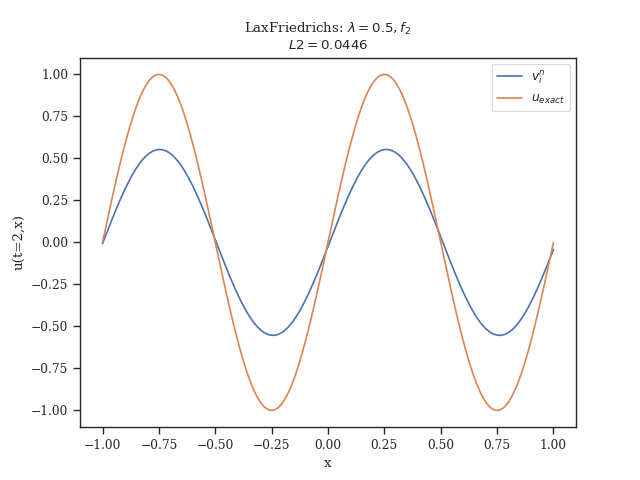
\includegraphics[width=\linewidth]{figures/LaxFriedrichs/LaxFriedrichs_lambda=0.5,f2}
        \caption{Lax-Friedrichs, $\lambda =0.5$}
    \end{subfigure}
    \hfill
    \begin{subfigure}{0.3\linewidth}
        \centering
        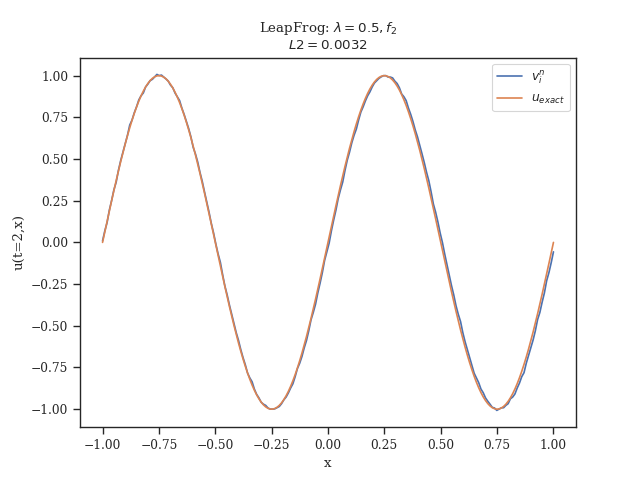
\includegraphics[width=\linewidth]{figures/LeapFrog/LeapFrog_lambda=0.5,f2}
        \caption{Leap-Frog, $\lambda =0.5$}
    \end{subfigure}
    \hfill
    \vspace{1cm}
    \begin{subfigure}{0.3\linewidth}
        \centering
        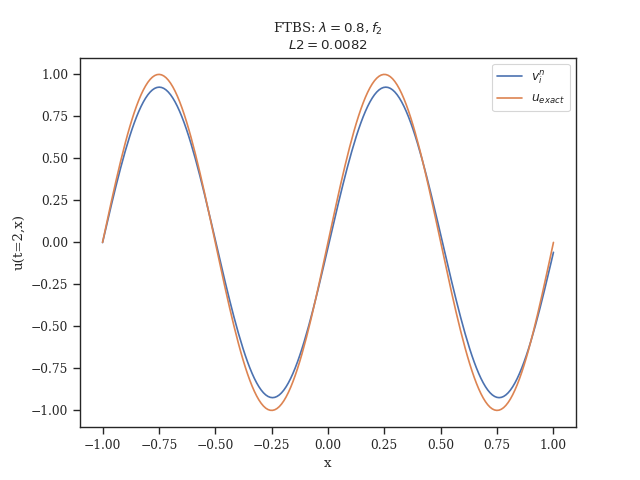
\includegraphics[width=\linewidth]{figures/FTBS/FTBS_lambda=0.8,f2}
        \caption{FTBS, $\lambda = 0.8$}
    \end{subfigure}
    \hfill
    \begin{subfigure}{0.3\linewidth}
        \centering
        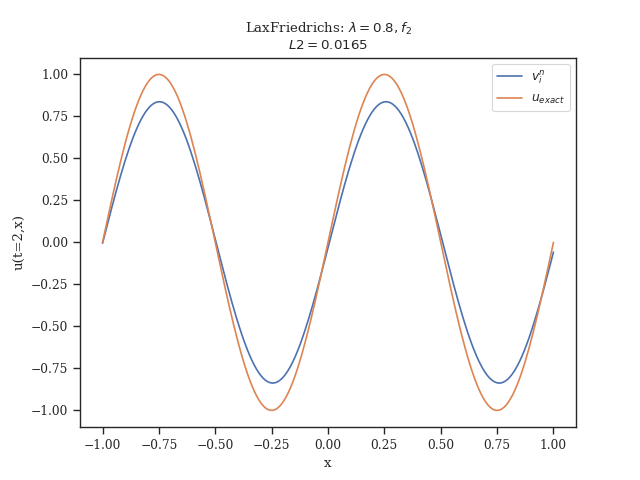
\includegraphics[width=\linewidth]{figures/LaxFriedrichs/LaxFriedrichs_lambda=0.8,f2}
        \caption{Lax-Friedrichs, $\lambda =0.8$}
    \end{subfigure}
    \hfill
    \begin{subfigure}{0.3\linewidth}
        \centering
        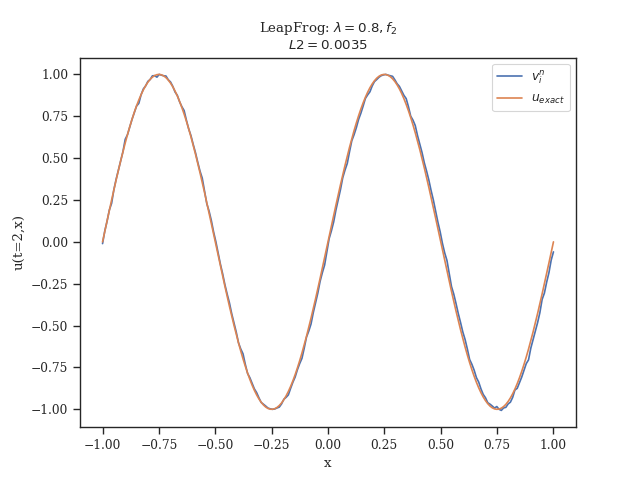
\includegraphics[width=\linewidth]{figures/LeapFrog/LeapFrog_lambda=0.8,f2}
        \caption{Leap-Frog, $\lambda =0.8$}
    \end{subfigure}
    \hfill
    \vspace{1cm}
    \begin{subfigure}{0.3\linewidth}
        \centering
        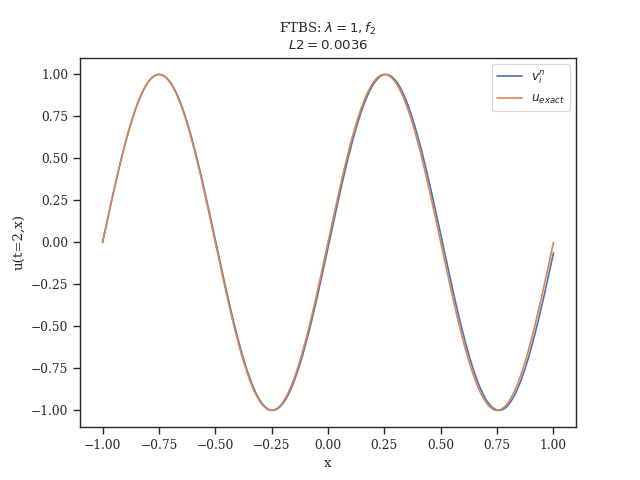
\includegraphics[width=\linewidth]{figures/FTBS/FTBS_lambda=1,f2}
        \caption{FTBS, $\lambda = 1$}
    \end{subfigure}
    \hfill
    \begin{subfigure}{0.3\linewidth}
        \centering
        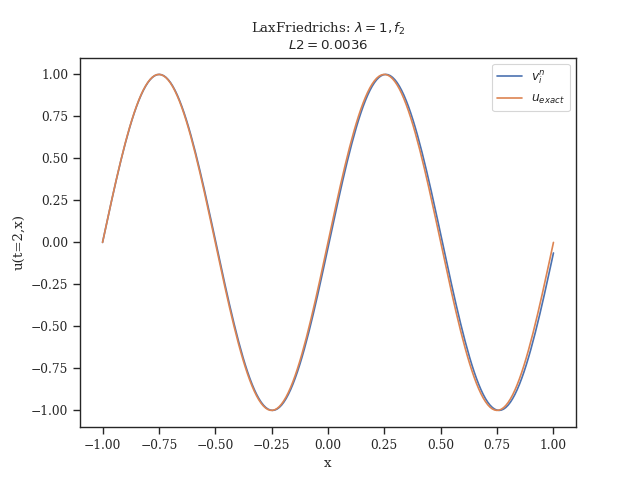
\includegraphics[width=\linewidth]{figures/LaxFriedrichs/LaxFriedrichs_lambda=1,f2}
        \caption{Lax-Friedrichs, $\lambda =1$}
    \end{subfigure}
    \hfill
    \begin{subfigure}{0.3\linewidth}
        \centering
        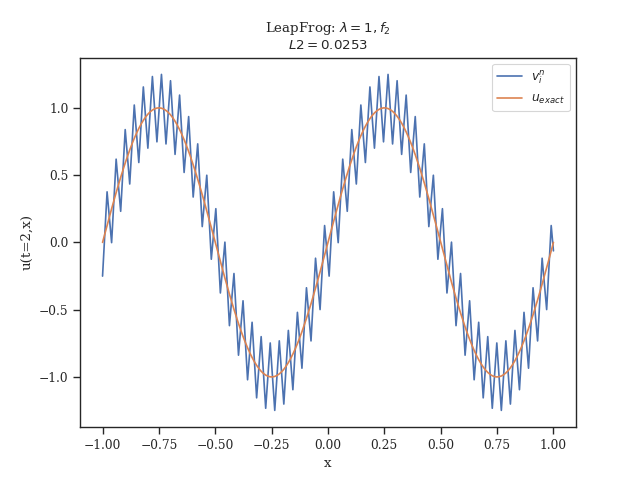
\includegraphics[width=\linewidth]{figures/LeapFrog/LeapFrog_lambda=1,f2}
        \caption{Leap-Frog, $\lambda =1$}
        \label{weird leap frog}
    \end{subfigure}
    \hfill
    \vspace{1cm}
    \begin{subfigure}{0.3\linewidth}
        \centering
        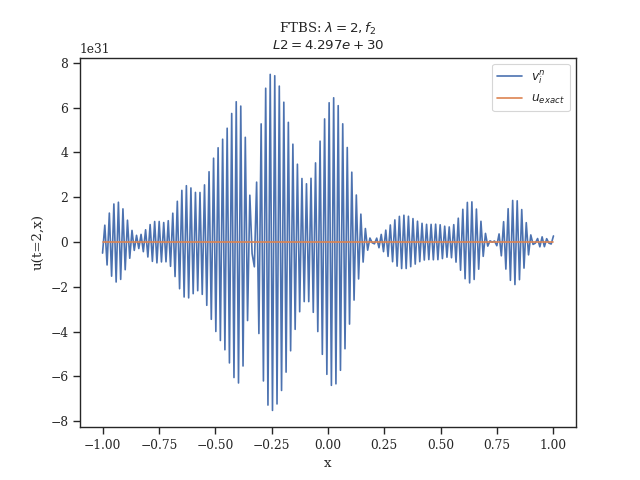
\includegraphics[width=\linewidth]{figures/FTBS/FTBS_lambda=2,f2}
        \caption{FTBS, $\lambda = 2$}
    \end{subfigure}
    \hfill
    \begin{subfigure}{0.3\linewidth}
        \centering
        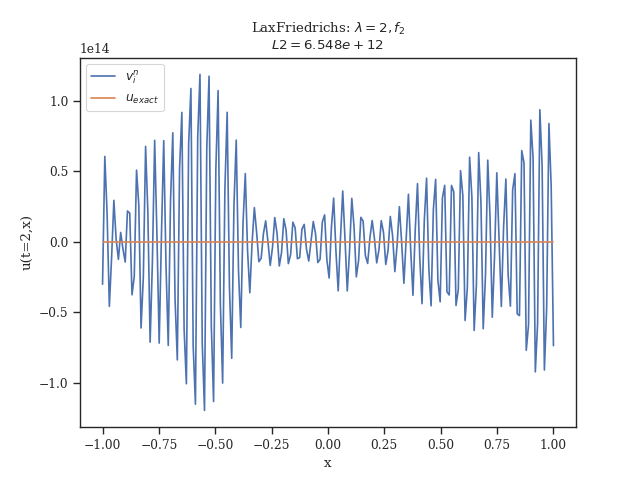
\includegraphics[width=\linewidth]{figures/LaxFriedrichs/LaxFriedrichs_lambda=2,f2}
        \caption{Lax-Friedrichs, $\lambda =2$}
    \end{subfigure}
    \hfill
    \begin{subfigure}{0.3\linewidth}
        \centering
        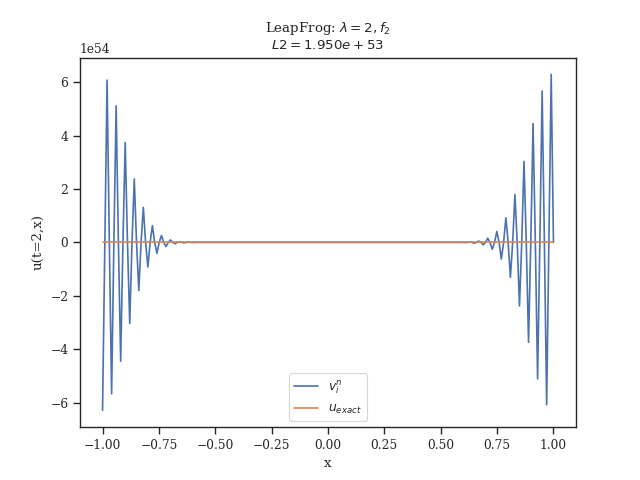
\includegraphics[width=\linewidth]{figures/LeapFrog/LeapFrog_lambda=2,f2}
        \caption{Leap-Frog, $\lambda =2$}
    \end{subfigure}
    \hfill

    \caption{Solutions of Varying $\lambda$ for $f_2$}
    \label{f2 figures}

\end{figure}
\appendix


%    \section{Python Code}
%    \inputminted[linenos, bgcolor=LightGray, fontsize=\footnotesize]{python}{578_HW1.py}
    
    \appendix
    \section{Code}
    \inputminted{python}{578_HW1.py}

\end{document}
